\begin{frame}{LR-E2E: Learn with a Rule-Consistency Loss}
    \small
    \textbf{Idea:} penalize predictions that conflict with active rules and update the model directly.

    \vspace{0.75em}
    \centering
    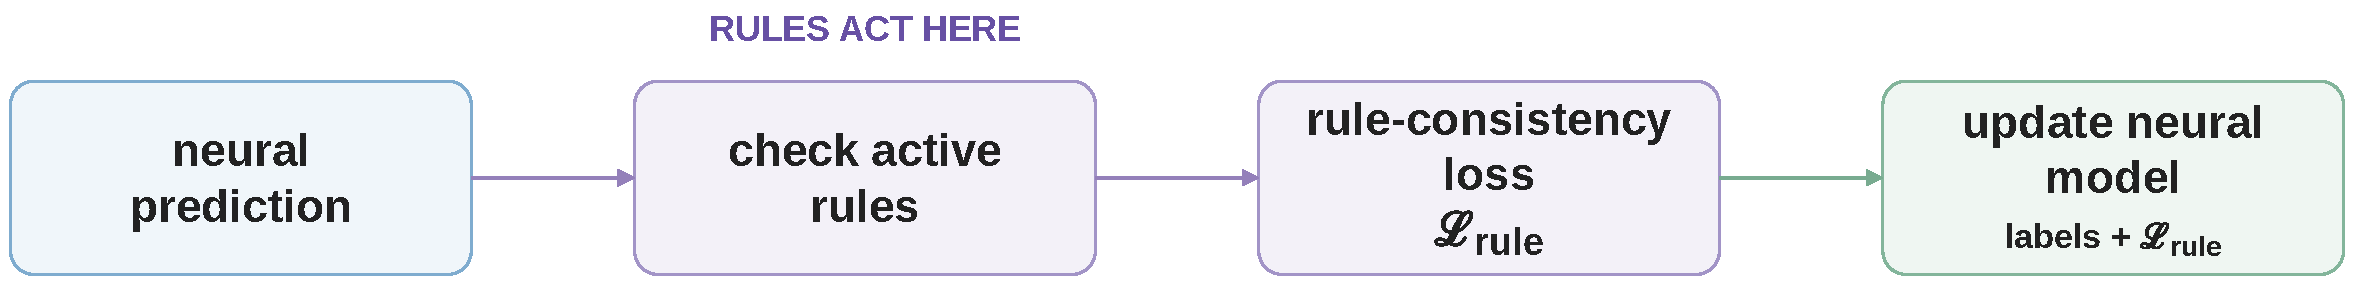
\includegraphics[width=0.94\linewidth]{figures/diagrams/lr_e2e.pdf}

    \vspace{0.85em}
    \begin{columns}[T,onlytextwidth]
        \column{0.48\linewidth}
        \begin{beamercolorbox}[wd=\linewidth,sep=0.6em,rounded=true]{defbox}
            \textbf{Model change}\par
            Neural parameters are updated by label and rule losses.
        \end{beamercolorbox}

        \column{0.48\linewidth}
        \begin{beamercolorbox}[wd=\linewidth,sep=0.6em,rounded=true]{takebox}
            \textbf{Deployment}\par
            Adapted neural model only; rules are no longer required.
        \end{beamercolorbox}
    \end{columns}
\end{frame}
